% ~ 6 pages
\chapter{The ATLAS Experiment at the Large Hadron Collider}
\label{chap:atlas}

The LHC at CERN is a symmetric proton--proton and heavy ion collider, supplying
collision events to four major experiments: ATLAS, CMS, ALICE and LHCb. In
proton--proton operation, bunches of protons are crossed at the interaction
points located inside of the experiments with a peak bunch crossing rate
of~\SI{40}{\mega\hertz}~\cite{lhc}. With a proton beam energy of \SI{6.5}{\TeV}
during Run~2 of the LHC, the proton--collisions take place at a center-of-mass
energy of \SI{13}{\TeV}. During the 2016 data taking period, a peak
instantaneous luminosity of~\SI{1.4e34}{\per\square\centi\metre\per\second} was
reached~\cite{lhc_2016_report}, which was further increased for the 2017 period.

\section{The ATLAS Detector}
\label{sec:atlas}

The ATLAS detector is a multipurpose particle detector experiment at the
LHC~\cite{atlas_detector}. An overview of the detector is given in
Figure~\ref{fig:atlas_detector}. Its cylindrical geometry provides almost
$4\pi$~coverage and forward-backward symmetry with respect to the nominal
interaction point. Specialised detector subsystems are arranged in concentric
layers around the beam axis, enabling the reconstruction of photons, electrons,
muons, taus and jets. Moreover, the detector coverage allows to reconstruct
missing transverse energy from weakly and non-interacting particles.

\begin{figure}[htb]
  \centering
  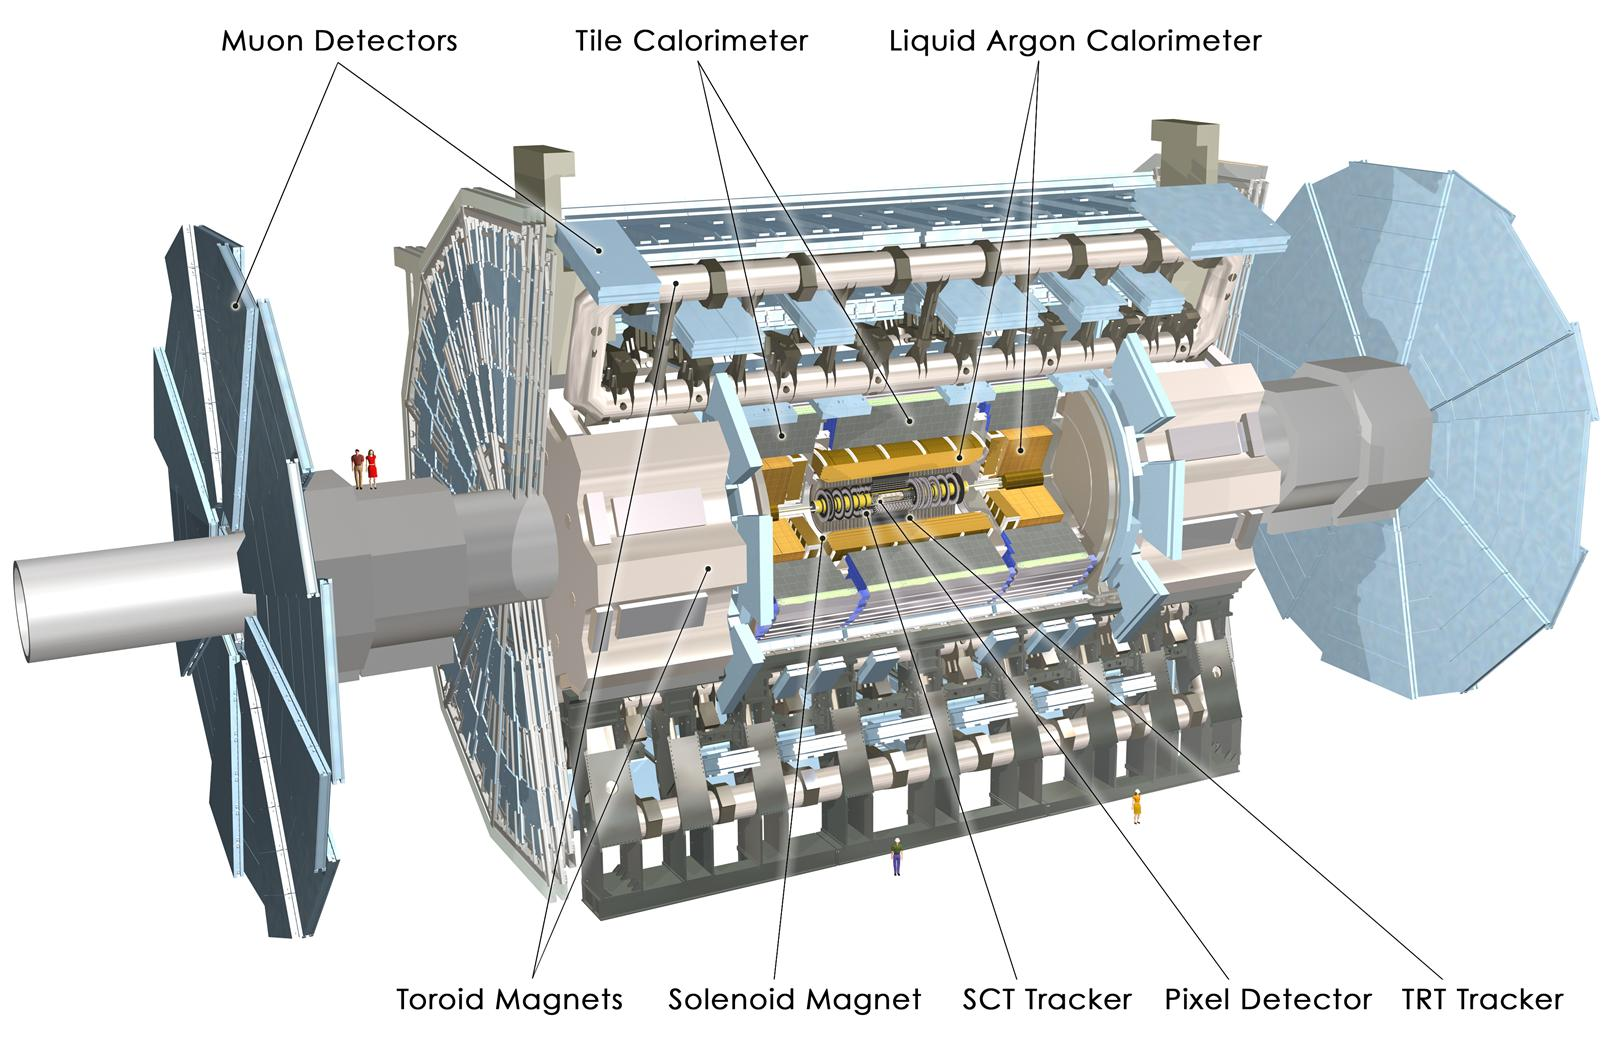
\includegraphics[width=0.8\textwidth]{./figures/atlas/overview.jpg}
  \caption{Overview of the ATLAS detector~\cite{atlas_detector}. Shown is the
    inner detector consisting of pixel, microstrip (SCT), transition radiation
    tracker (TRT) and solenoid; the calorimeter system consisting of LAr and
    Tile sampling calorimeters and the muon spectrometer consisting of tracking
    chambers and air-core toroids.}
  \label{fig:atlas_detector}
\end{figure}

In the ATLAS experiment a right-handed coordinate system is used to describe
positions in the detector. The origin of the coordinate system is located at the
nominal interaction point, with the $z$-axis pointing along the beam axis, the
$x$-axis towards the centre of the LHC ring and the $y$-axis upwards. The $x$-
and $y$-axes span the transverse plane. Spherical
coordinates~$(r, \varphi, \theta)$ are commonly used, with the azimuthal
angle~$\varphi$ being measured in the transverse plane and the polar
angle~$\theta$ with respect to the beam axis.

Due to the unknown longitudinal momentum of colliding partons in the
proton--proton collisions, the momentum of final state particles only balances
in the transverse plane. Therefore, transverse quantities for momentum and
energy are defined as
\begin{align*}
  p_\text{T} &= |\mathbf{p}| \sin\theta & E_\text{T} &= E \sin\theta \eqdot
\end{align*}
In addition, the unknown boost along the $z$-axis motivates the definition of
the pseudorapidity
\begin{align*}
  \eta &= -\ln\left[ \tan\left( \frac{\theta}{2} \right) \right] \eqcomma
\end{align*}
such that differences in~$\eta$ are Lorentz-invariant in the massless limit, and
the angular distance
\begin{align*}
  \Delta R &= \sqrt{\left(\Delta\eta\right)^2 + \left(\Delta\varphi\right)^2} \eqcomma
\end{align*}
where $\Delta \eta$ and $\Delta \varphi$ are the differences in pseudorapidity
and azimuthal angle, respectively.

In the following a brief description of the detector subsystems is given. In
increasing radial distance, the systems are:
\begin{description}
\item[Inner Detector] The inner detector (ID) consists of several layers of
  pixel detectors, silicon microstrip detectors and straw chambers. The ID is
  embedded in a \SI{2}{\tesla} axial magnetic field, bending the trajectories of
  charged particles in the transverse plane and allowing transverse momentum
  measurements. Hits of charged tracks in the active layers of the ID are
  reconstructed as so called space points, which are used to perform tracking
  and vertexing. The straw tubes of the Transition Radiation Tracker (TRT) offer
  tracking at large radii as well as electron identification via high-threshold
  hits originating from transition radiation of electrons crossing the tube
  material.

\item[Calorimeter System] The sampling calorimeters used in the ATLAS detector
  allow to measure the energies of photons, electrons and hadrons. The
  calorimeter system consists of an electromagnetic calorimeter with high
  granularity, designed to reconstruct energy depositions of photons and
  electrons, and the coarser hadronic calorimeter to reconstruct jets of
  hadrons.

\item[Muon Spectrometer] Muons passing the calorimeter are measured in
  high-precision tracking chambers in the magnetic field of an air-core toroid.
  The spectrometer allows to identify muons and measure their momentum from the
  curvature of reconstructed tracks in the muon system.

\item[Trigger and Data Acquisition Systems] The peak event rate of
  \SI{40}{\mega\hertz} in the ATLAS detector, mostly consisting of events not of
  immediate interest for physics research, needs to be reduced in a trigger
  system to match the limited throughput of the data acquisition systems, while
  still being sensitive to rare physics processes. The trigger of the ATLAS
  detector is divided into three levels: L1, L2 and the event filter. They
  successively reduce the rate, while having access to detector information of
  increasing granularity. After the final trigger level, the event filter, the
  rate is sufficiently small, such that events can be moved to permanent storage
  for later analysis.
\end{description}
For the reconstruction of hadronic tau decays, the tracking and calorimeter
systems are of large importance. In the following they are described in more
detail.

\section{Inner Detector}
\label{sec:atlas_tracking}

The inner detector of the ATLAS experiment provides track reconstruction in the
high particle density environment of proton--proton collisions at the LHC. This
allows to meet transverse momentum and vertex resolution requirements needed to
perform physics analyses. An overview of the inner detector is shown in
Figure~\ref{fig:atlas_indet}.

\begin{figure}[htb]
  \centering
  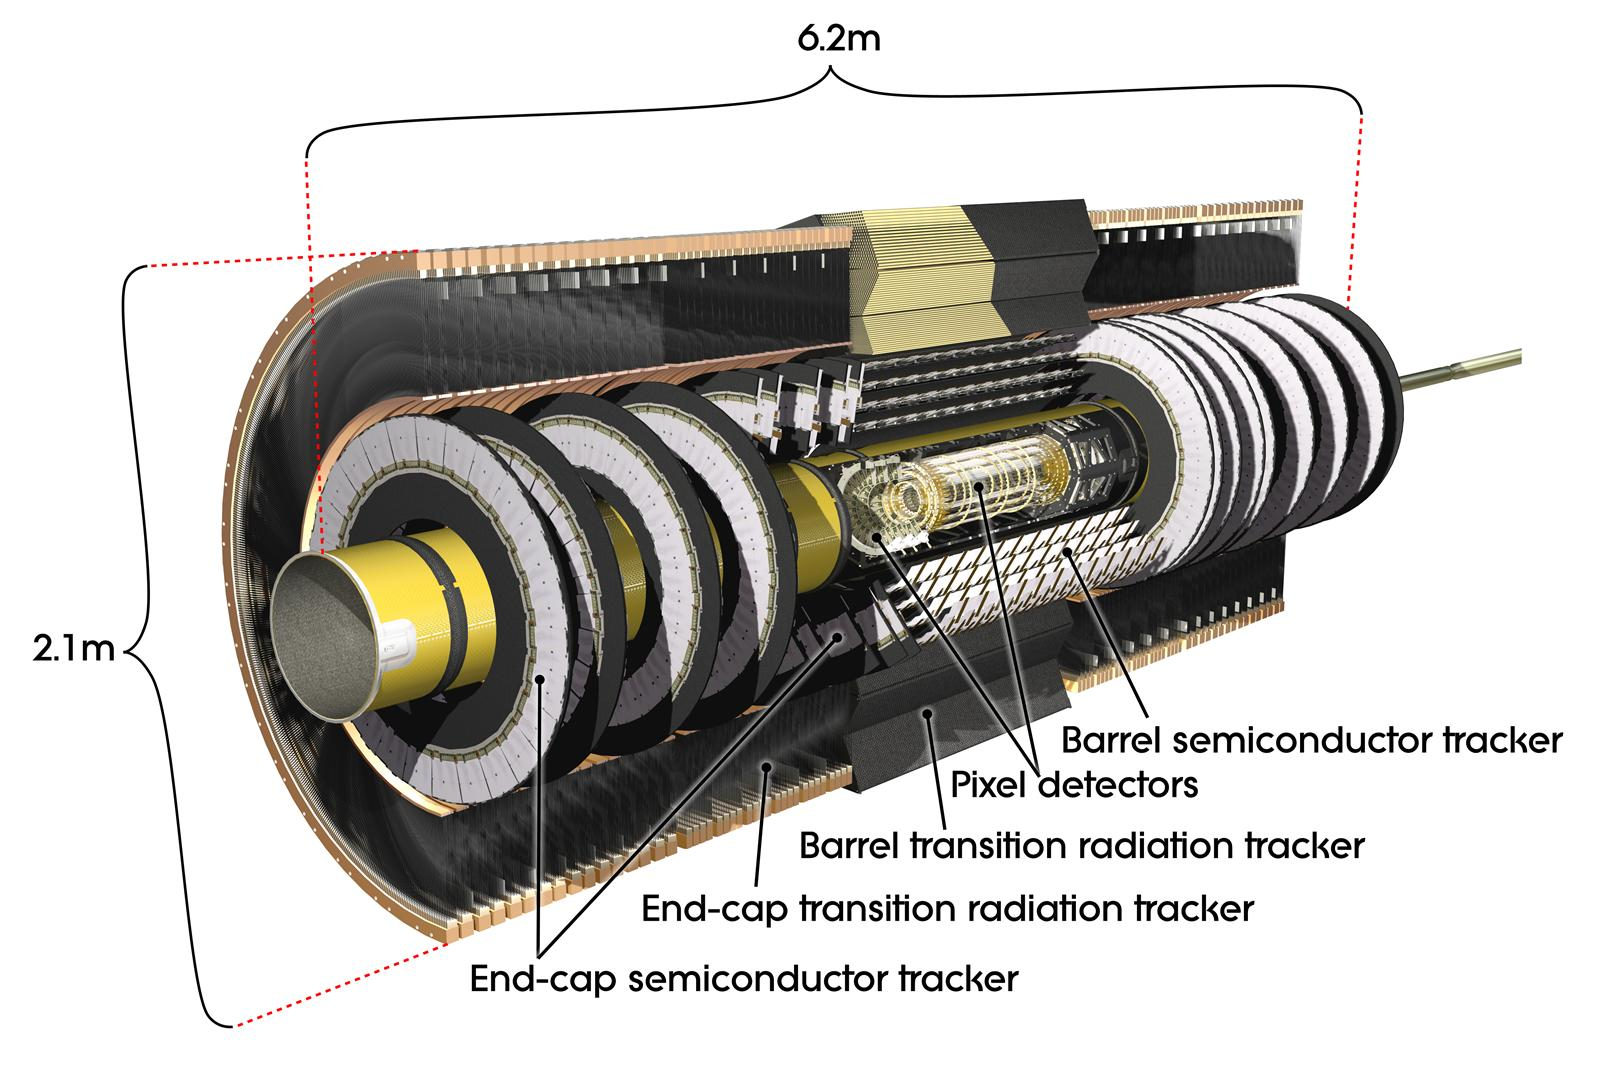
\includegraphics[width=0.75\textwidth]{./figures/atlas/inner_detector.jpg}
  \caption{Overview of the ATLAS inner detector~\cite{indet_fig}. Shown are
    pixel and, microstrip detector as well as the Transition Radiation Tracker.
    The innermost pixel layer, the Insertable B-Layer installed during
    Long~Shutdown~1, is not depicted.}
  \label{fig:atlas_indet}
\end{figure}

The inner detector consists of three distinct and complementary parts employing
different detector technologies. From the interaction point outwards, it
consists of: pixel detectors, silicon microstrip detectors and a transition
radiation detector using drift tubes.

The pixel detectors consist of the Insertable B-Layer (IBL), installed during
Long~Shutdown~1 at a reduced distance from the interaction point
of~$r = \SI{33.25}{\milli\metre}$~\cite{ibl_tdr}, and three additional layers
spanning radial distances from \SI{50.5}{\milli\metre} to
\SI{122.5}{\milli\metre}~\cite{atlas_detector} in the barrel of the ATLAS
detector. Additionally, three disks of pixel detectors cover the forward and
backward regions in two endcaps. The sensors of the IBL provide an intrinsic
resolution of approximately \SI{10}{\micro\metre} in the azimuthal ($r\varphi$)
direction and \SI{65}{\micro\metre} in $z$-direction~\cite{ibl_measurement}. The
other layers have resolutions of \SI{10}{\micro\metre} in $r\varphi$ and
\SI{115}{\micro\metre} in $z$-direction~\cite{atlas_detector}. The high
resolution of the pixel detectors and their proximity to the interaction point
are crucial for track impact parameter measurements (cf.\
Figure~\ref{fig:impact_params}) and for primary as well as secondary vertex
reconstruction.

\begin{figure}[htb]
  \begin{subfigure}[t]{0.48\textwidth}
    \centering
    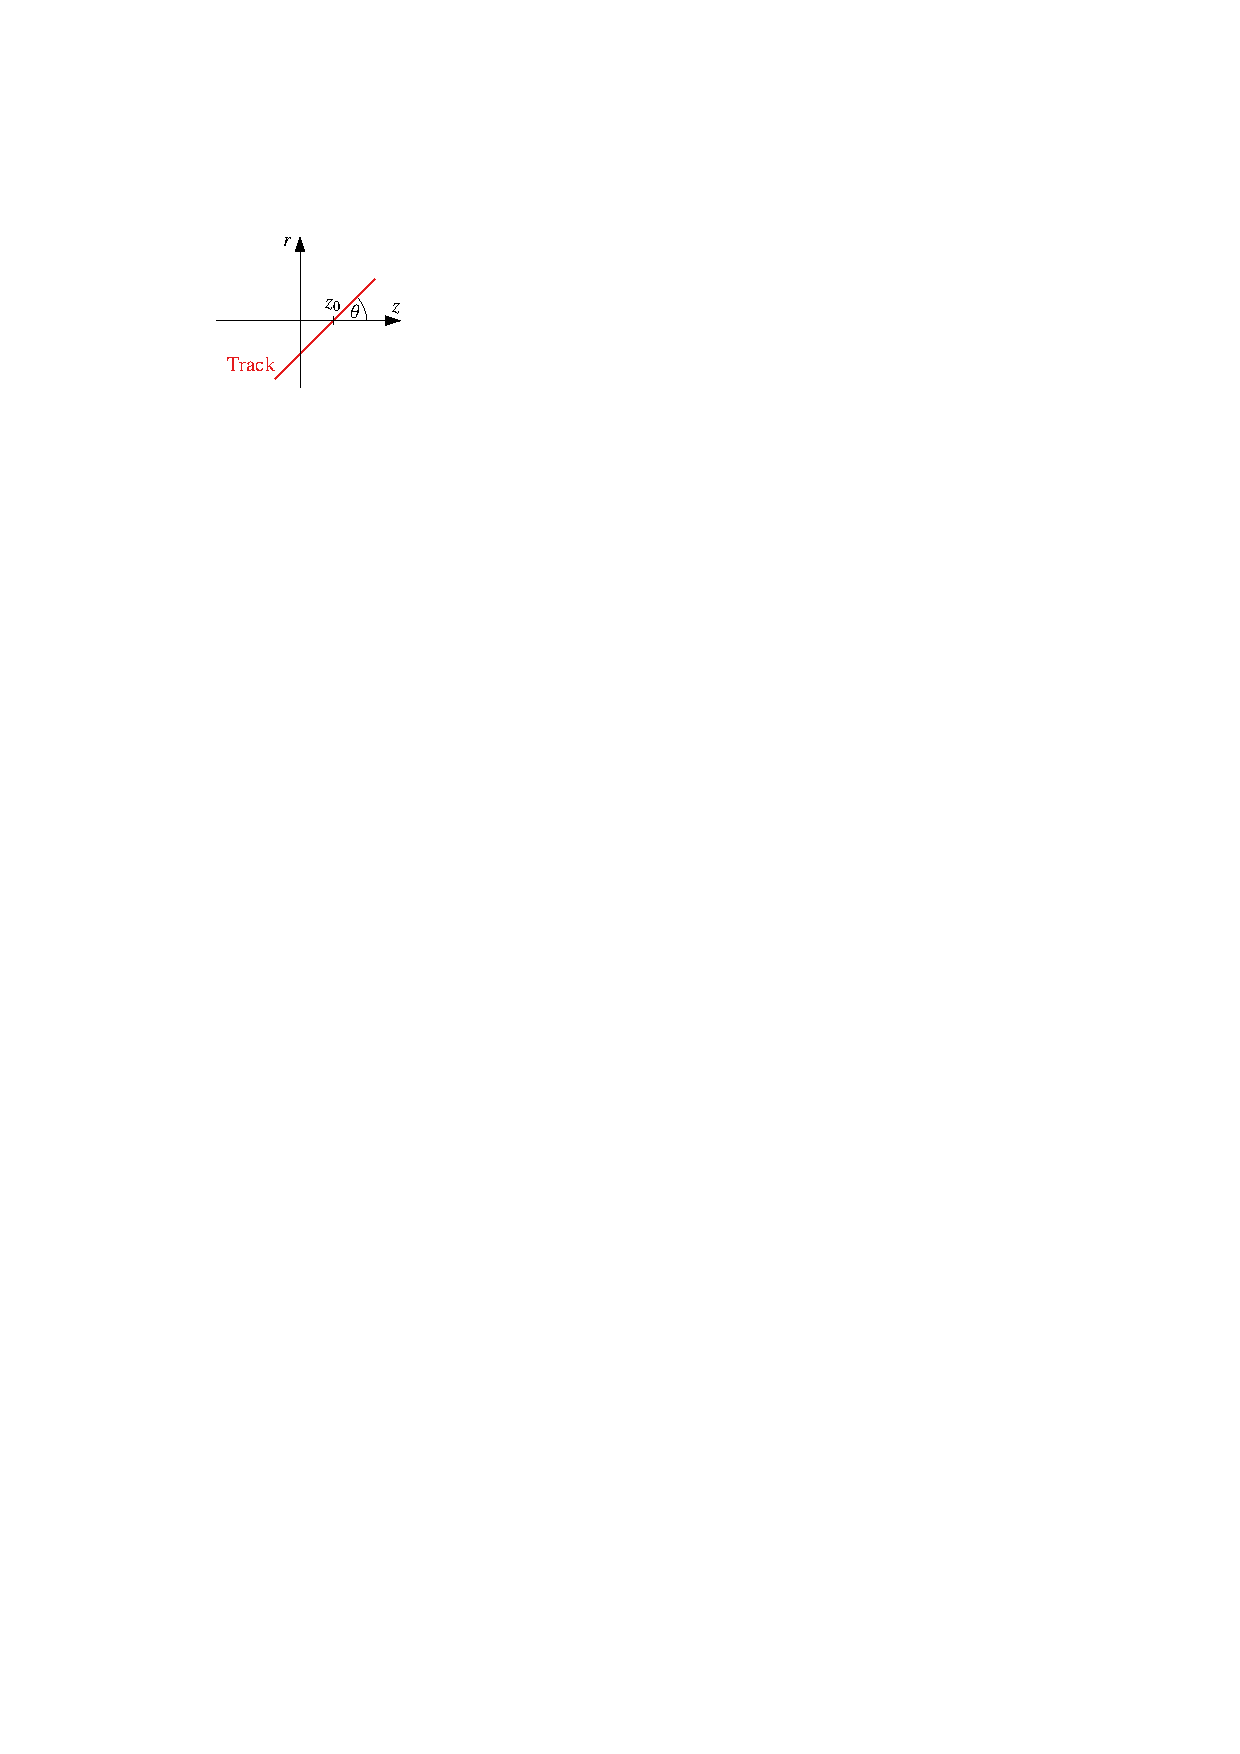
\includegraphics{./figures/atlas/impact_params_z0.pdf}
    \subcaption{Definition of the longitudinal impact parameter, $z_0$.}
    \label{fig:longitudinal_impact_param}
  \end{subfigure}\hfill
  \begin{subfigure}[t]{0.48\textwidth}
    \centering
    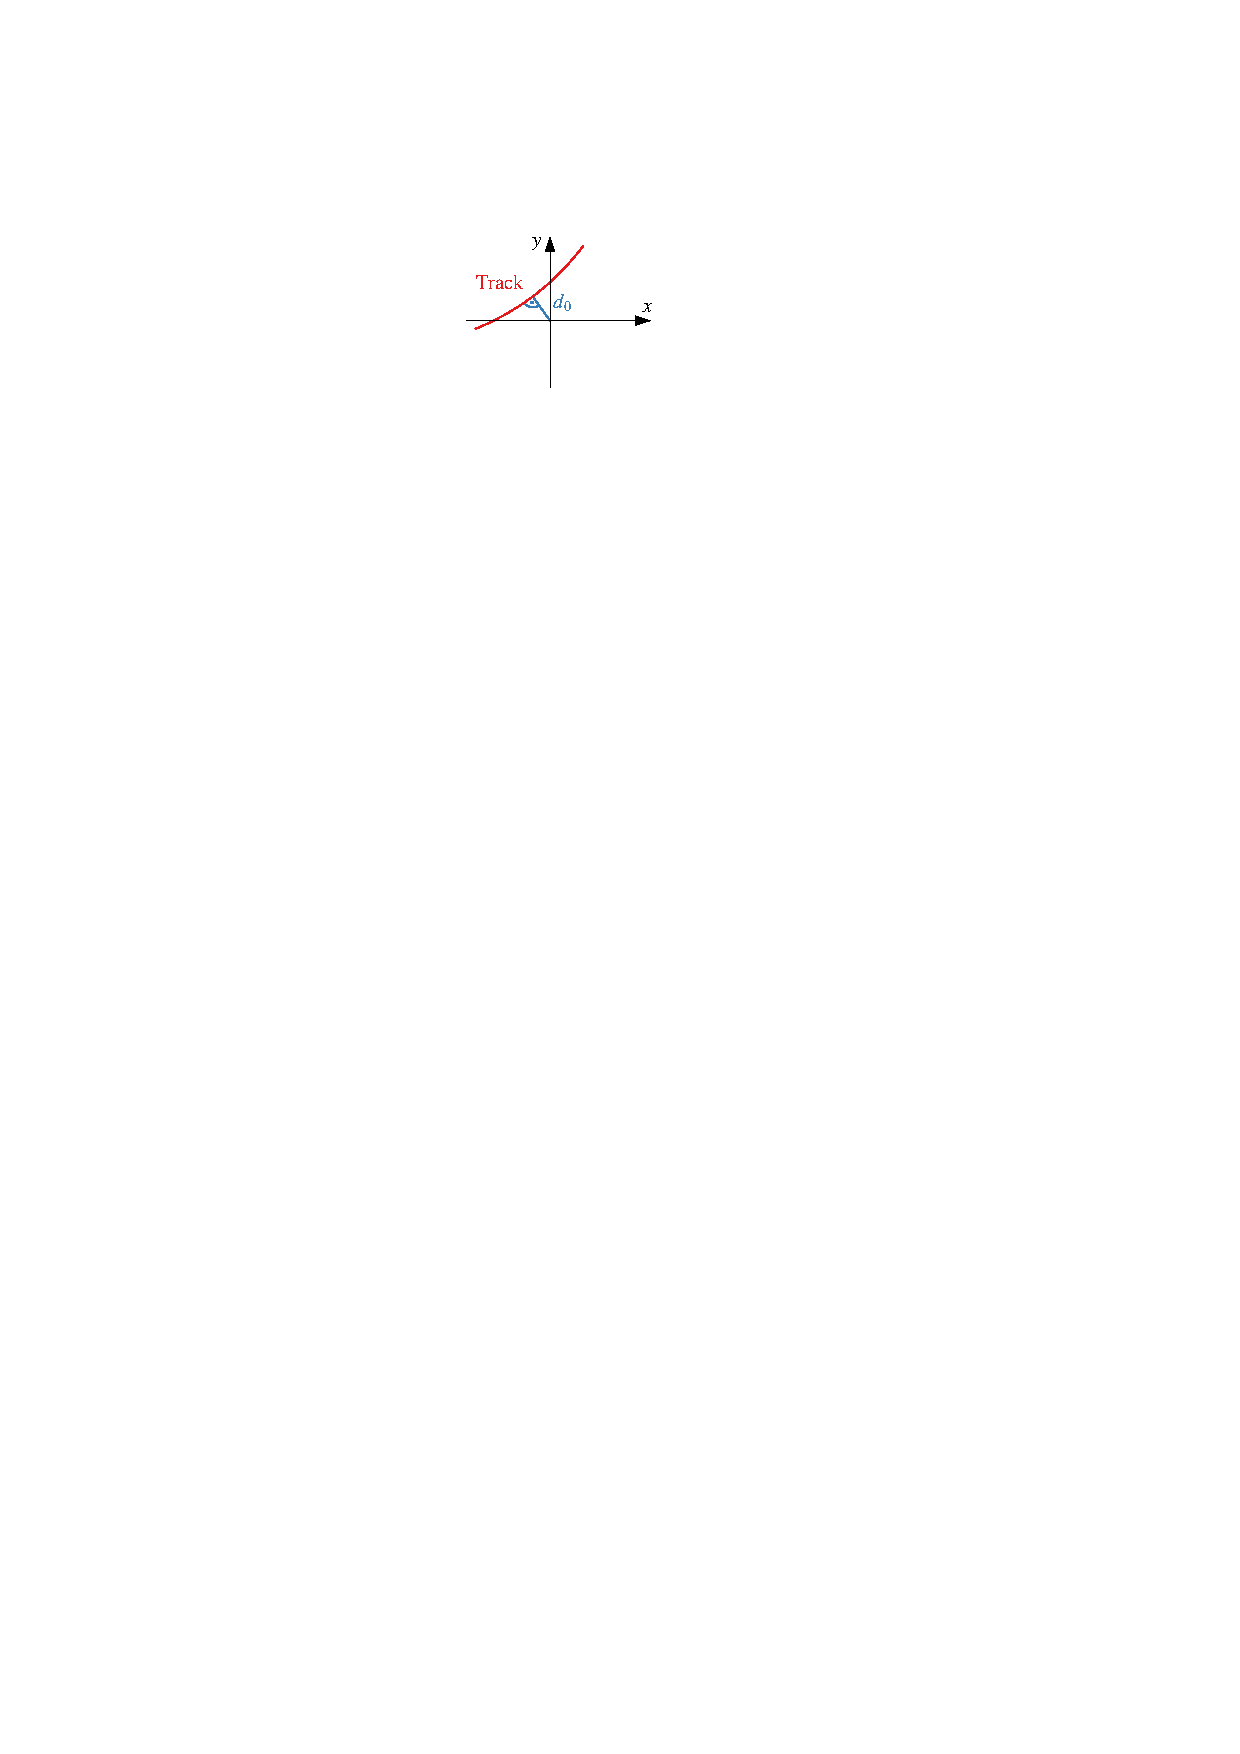
\includegraphics{./figures/atlas/impact_params_d0.pdf}
    \subcaption{Definition of the transverse impact parameter, $d_0$. The sign
      of $d_0$ depends on the angular momentum of the track w.r.t.\ the
      reference.}
    \label{fig:transverse_impact_param}
  \end{subfigure}
  \caption{Definitions of the impact parameters at the perigee with respect to a
    reference point (here at the origin).}
  \label{fig:impact_params}
\end{figure}

The Semiconductor Tracker (SCT) is a silicon microstrip detector with four
barrel layers covering the intermediate radial range from
$r = \SI{299}{\milli\metre}$ to \SI{514}{mm}~\cite{atlas_detector}. In the
endcaps the SCT consists of nine disks perpendicular to the beam axis. The
intrinsic resolution of the SCT sensors is \SI{17}{\micro\metre} in $r\varphi$
and in axial (radial) direction \SI{580}{\micro\metre} for barrel
(disks)~\cite{atlas_detector}. The tracking detectors based on semiconductor
technology provide a pseudorapidity coverage of approximately~$|\eta| < 2.5$.

Track measurement at large radial ranges of $r = \SI{554}{\milli\metre}$ to
\SI{1082}{\milli\metre} are provided by the TRT consisting of drift tubes with a
diameter of \SI{4}{\milli\metre} aligned with the beam axis. As a result, they
only provide azimuthal measurements with an intrinsic resolution of
\SI{130}{\micro\metre}~\cite{atlas_detector}. With a large number of 73 (160)
straw planes in the barrel (endcap) it provides nearly continuous tracking and
electron identification over a pseudorapidity range
of~$|\eta| < 2.0$~\cite{atlas_detector}.

Charged-particle tracks are reconstructed from space points using sophisticated
pattern-recognition and tracking algorithms. After reconstruction, several
representations can be used to define tracks. In the ATLAS detector, tracks are
often represented at the perigee with respect to a reference point, which is
commonly the primary vertex or the beamspot. In this representation tracks are
unambiguously defined by the transverse and longitudinal impact parameters,
$d_0$ and $z_0$ (cf.\ Figure~\ref{fig:impact_params}), the azimuthal and polar
angles of the track momentum at the perigee, $\varphi$ and $\theta$, as well as
the ratio of charge and momentum of the track, $q / p$.


% See \url{https://twiki.cern.ch/twiki/bin/view/AtlasProtected/InDetTrackingDC14#Impact_parameters_z0_d0_definiti}


\section{Calorimeter System}
\label{sec:atlas_calo}

\todo[inline]{Topoclustering}
\todo[inline]{Define what a moment is}
\todo[inline]{EM and LC scale}
\todo[inline]{Introduce nomenclature: strip layer, EM1, EM2, EM3, HAD}

Coverage:

EM LAr covers $|\eta|< 3.2$

Scintillator-tile in~$|\eta| < 1.7$

End-caps hadronic $|\eta| > 1.5$ also LAr coverage to $|\eta| = 4.9$

\begin{figure}[ht]
  \centering
  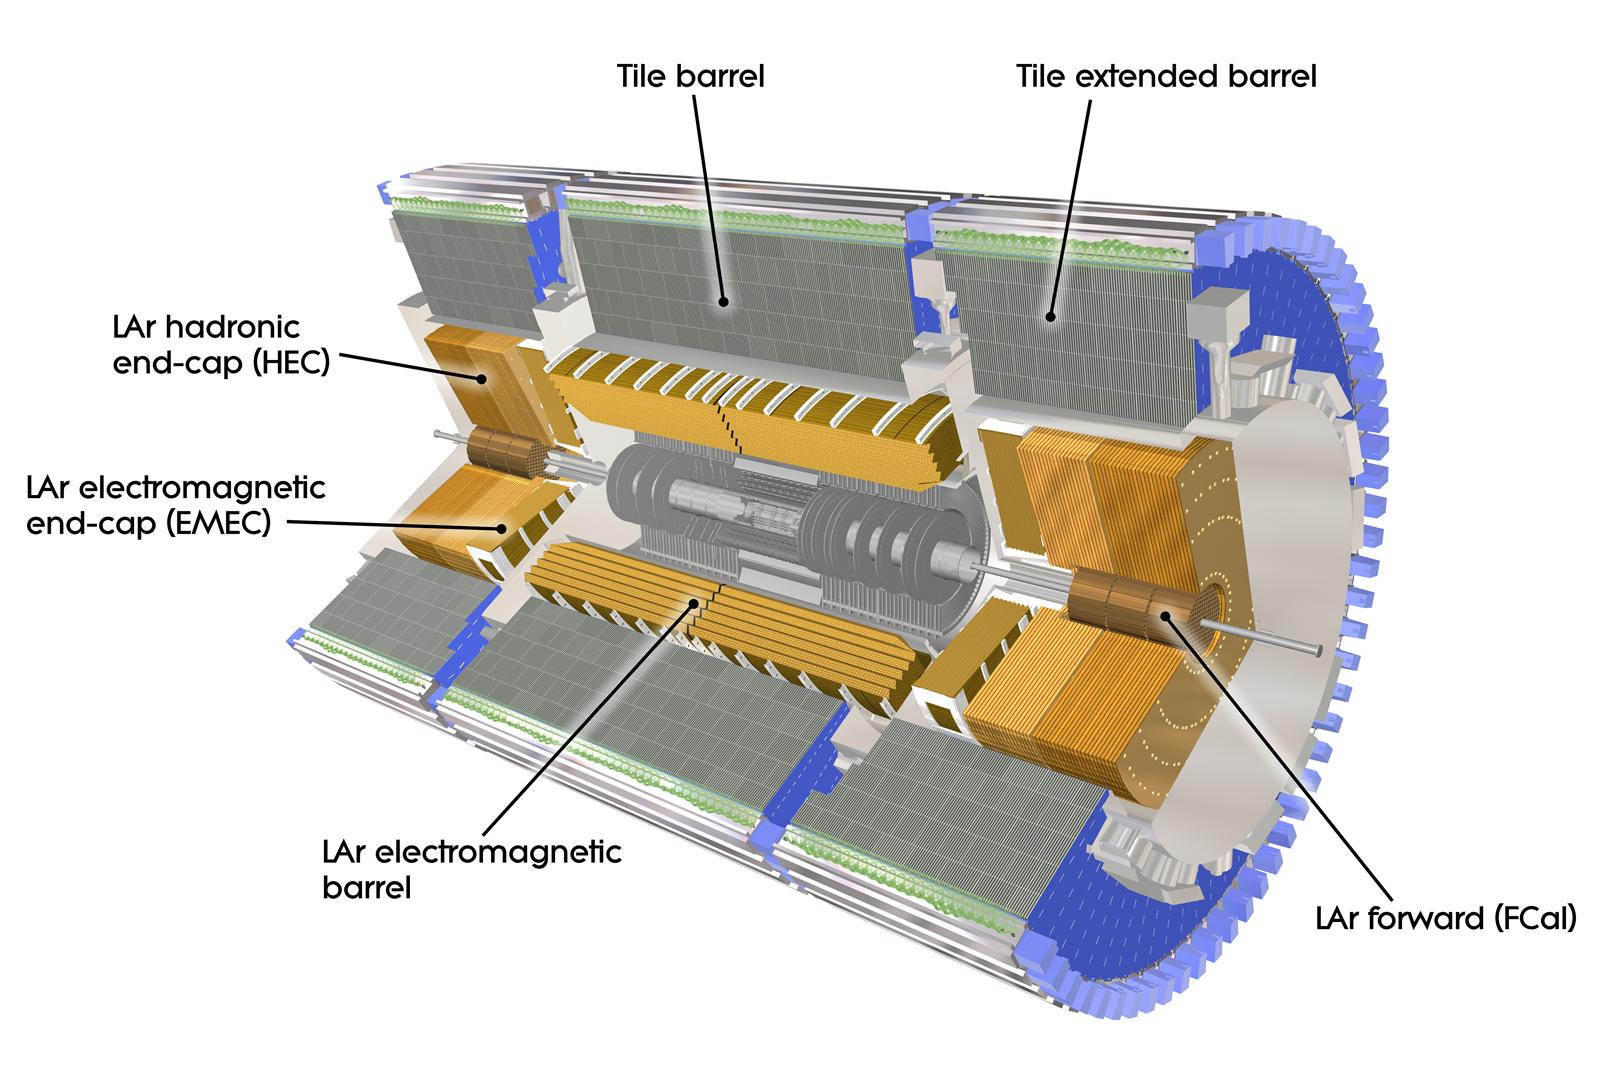
\includegraphics[width=0.8\textwidth]{./figures/atlas/calorimeter.jpg}
  \caption{ATLAS calorimeter\cite{calo_fig} also in \cite{atlas_detector}}
  \label{fig:atlas_indet}
\end{figure}



\begin{itemize}
\item LHC (brief)

\item ATLAS
  \begin{itemize}
  \item Overview (Design goals) \\
    brief: Beam Line, Inner Detector \& Solenoid, Calorimeter, Muon System \&
    Toroid, Trigger

  \item Nomenclature (Coordinate system, Pseudorapidity, $\Delta R$,
    $p_\mathrm{T}$)

  \item Inner detector / Tracker (and why they are important for taus)
    \begin{itemize}
    \item Pixel, IBL
    \item SCT
    \item TRT
    \item  Transverse Momentum Resolution, Vertex \& Secondary Vertex
      reconstruction, Impact Parameter Resolution, $\eta$-Coverage
    \end{itemize}

  \item Calorimeter (and why they are important for taus)
    \begin{itemize}
    \item Presampler, LAr (EM1 - EM3), Had (Tile, LAr)
    \item Cell sizes, $\eta$-Coverage, Thickness $X_0$ / $\lambda$,
      Energy Resolution vs. $E$
    \item Topoclusters \& Cluster moments
    \end{itemize}

  \end{itemize}
\end{itemize}

%%% Local Variables:
%%% mode: latex
%%% TeX-master: "mythesis"
%%% End:
